\section{実機実験}
本章では製作したロボットを用いて行った実機実験について述べる.

\subsection{乗り上げる動作の検証}
ロボットが他のロボットに乗り上げることが実現できるかどうかを実機検証した.
\reffig{climb}から,ロボットが3段まで乗り上げられることが確認できた.
\begin{figure}[tb]
  \centering
  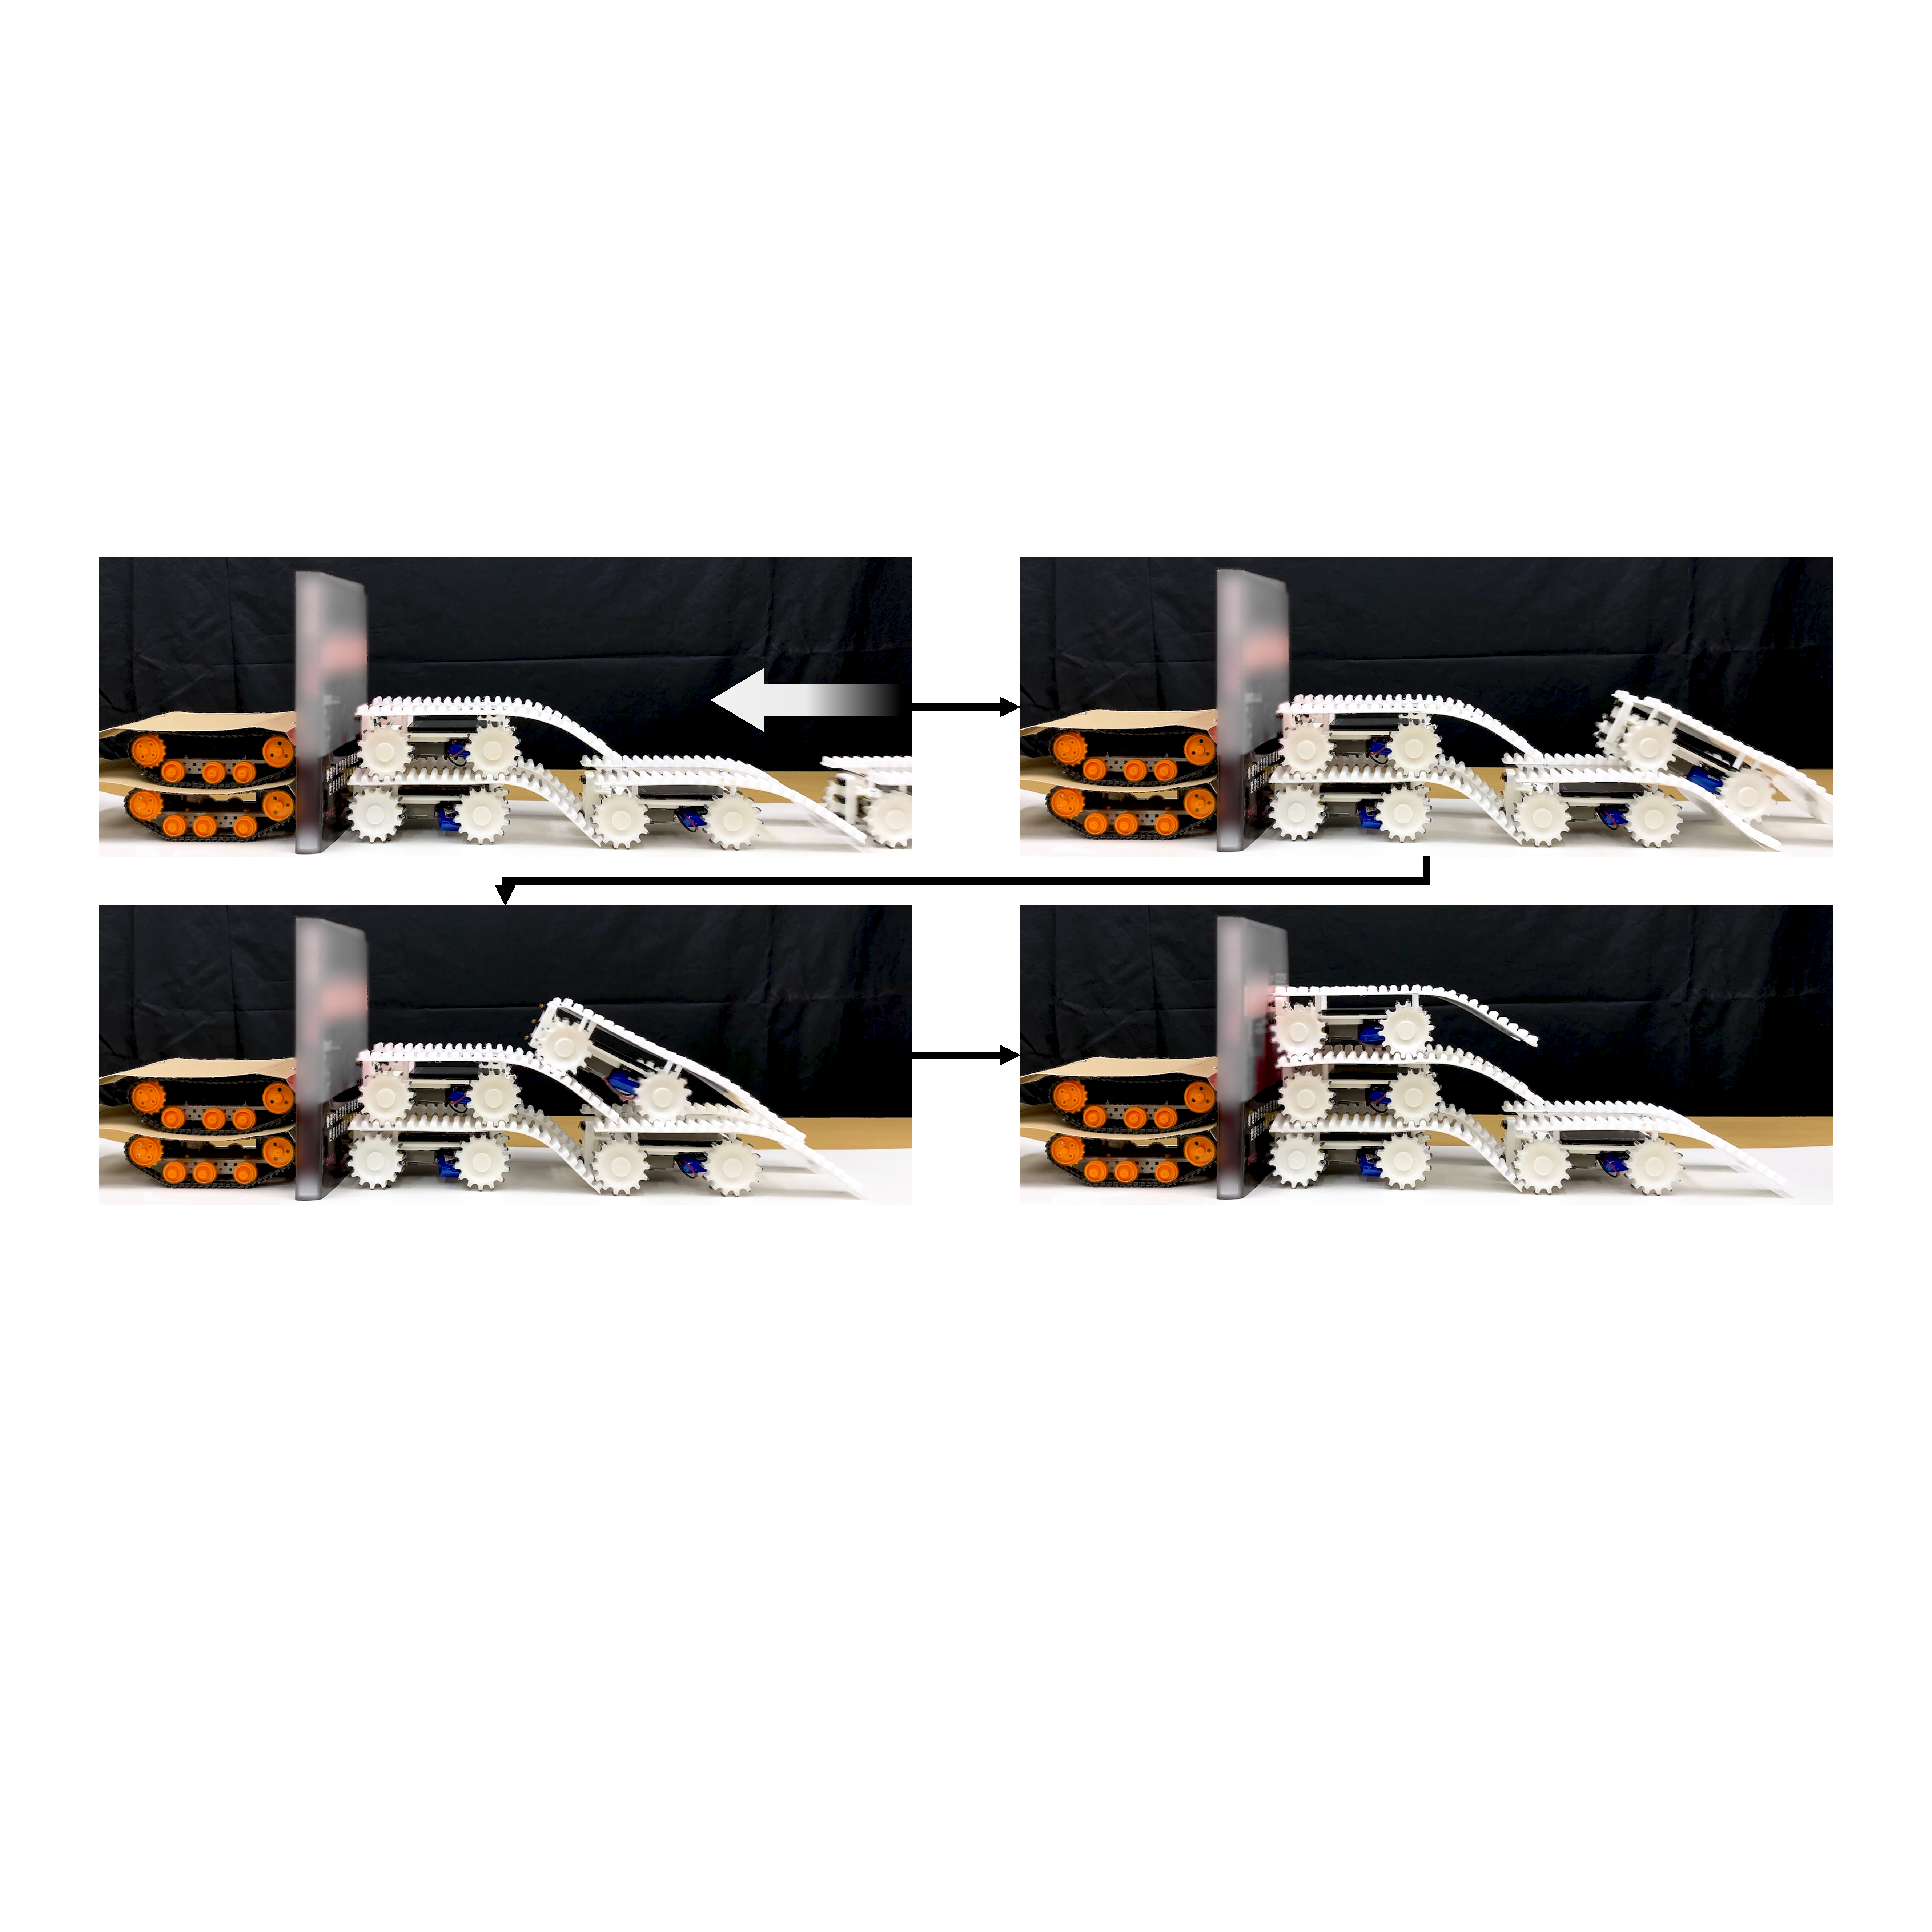
\includegraphics[width=\columnwidth]{figures/climb.pdf}
  \caption{Experiment of climbing}
  \label{fig:climb}
\end{figure}

\begin{figure}[tb]
  \centering
  \includegraphics[width=0.85\columnwidth]{figures/pulling-mechanism.pdf}
  \caption{Pulling mechanism}
  \label{fig:pulling-mechanism}
\end{figure}
\subsection{段数の変更による物体の安定化性能に関する実験}
次に,移動ロボットが移動しているとき,支持部のロボットが物体を支持できるかどうかを確認した.
ここからの実験は提案システムの移動部をロボットの代わりとして,紙を使用した.
また,紙を一定力で引っ張るために,\reffig{pulling-mechanism}に示すような牽引装置を作成した.
牽引装置はTAMIYA社のキャタピラ車をワイヤで机に前進しないように固定し,安定化電源で一定の電圧をかける. このとき,クローラーが摩擦よって,紙を送り出し,紙の上に載せているものを一定速度で動かすことができる.

上述の牽引装置を利用し,搬送物体として本を立てて置いた.その両側にロボットを1段ずつと2段ずつ置き,牽引装置に6~Vの電圧を印加したときの安定化性能の比較を行った.
\reffig{1layer}から,1段の場合では紙を送り出すと物体は倒れた.
しかし,\reffig{2layer}から,2段の場合では紙を送り出してから止まるまで物体は初期姿勢を保つことができた.
その原因として,牽引装置の印加電圧が6~Vのとき,全体の加速度が大きいため,1段で支持する場合はロボットが滑ってしまい,物体を支持できなくなる.しかし,2段に増やすと,物体の重心近くで支持することと,2段のロボットが紙から滑りにくくなることによって,物体を支持し移動することができたと考えられる.
\begin{figure}[tb]
  \centering
  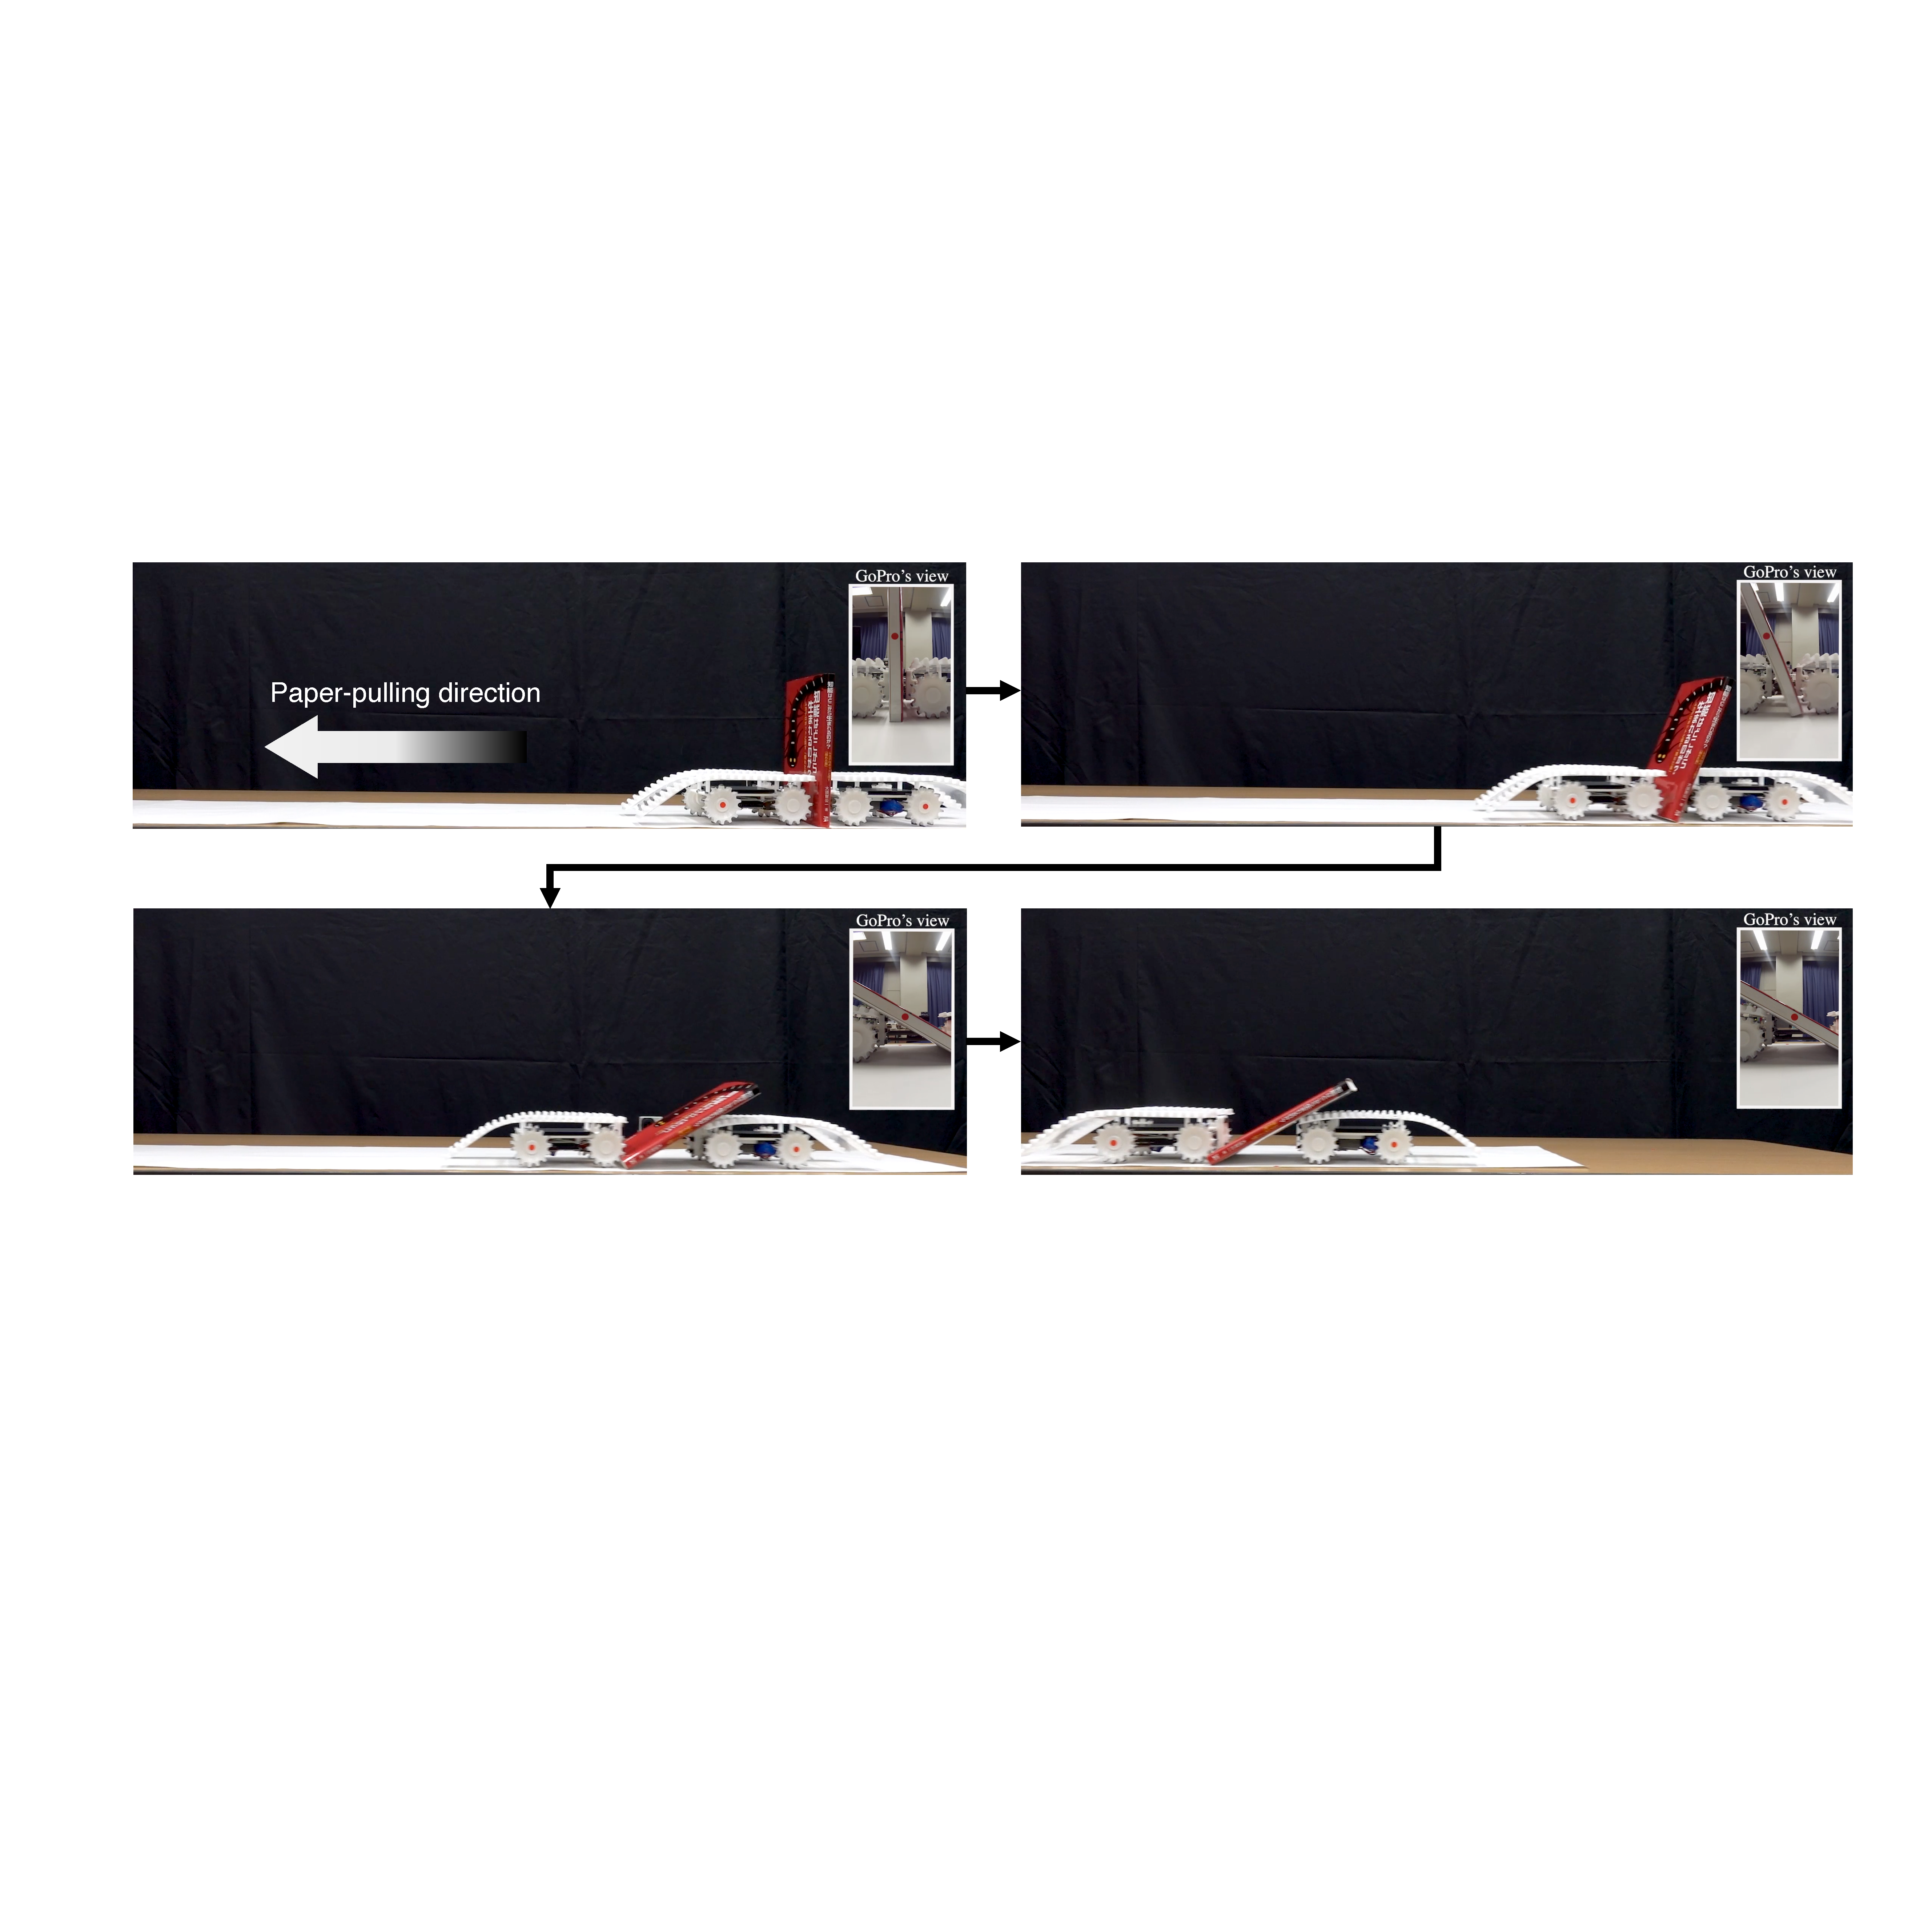
\includegraphics[width=\columnwidth]{figures/1layer.pdf}
  \caption{Experiment of supporting with 1 layer}
  \label{fig:1layer}
\end{figure}
\begin{figure}[tb]
  \centering
  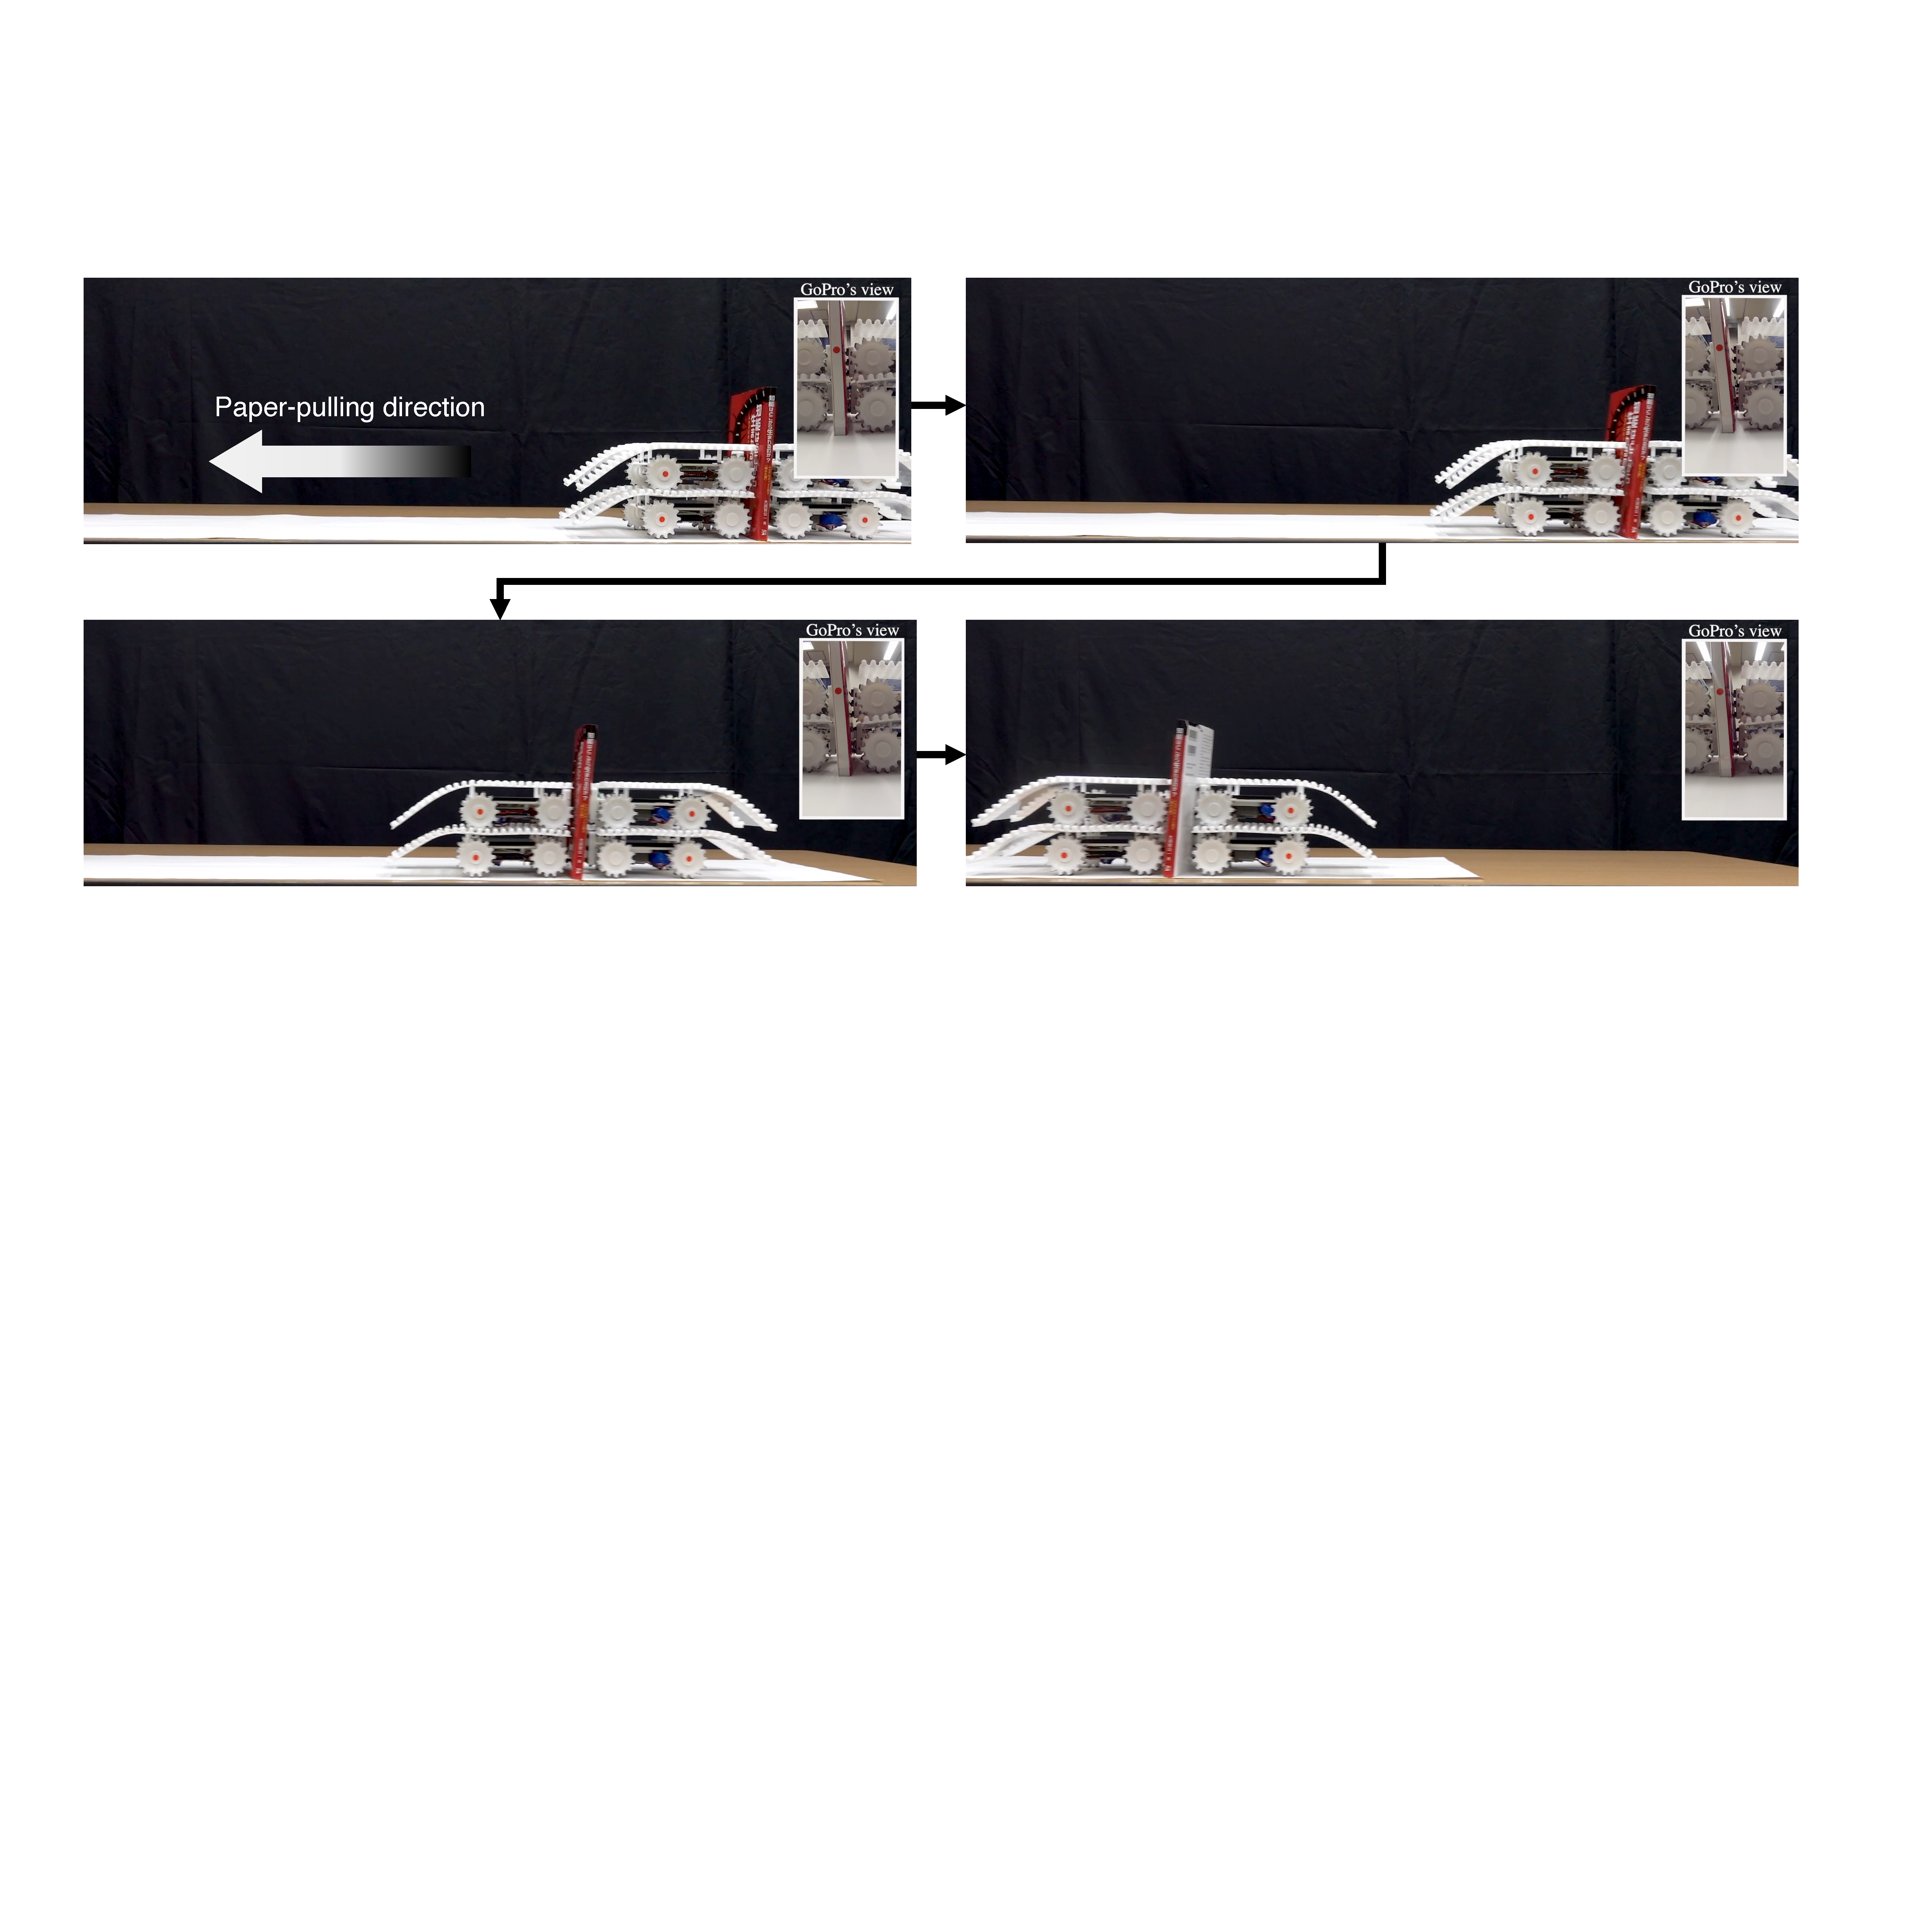
\includegraphics[width=\columnwidth]{figures/2layers.pdf}
  \caption{Experiment of supporting with 2 layers}
  \label{fig:2layer}
\end{figure}

\subsection{制御による物体の安定化性能に関する実験}
製作したロボットの物体の姿勢を検知するセンサを利用し,物体の初期姿勢に戻そうとする制御をかけると,前節では物体を支持することができなかったロボットが1段の場合でも,物体を支持できるかを確認する実験を行った.
まず,\reffig{control-figure}に示すようにかける制御について述べる.\reffig{upright}より,センサの上下両方のスイッチが反応したとき,ロボットに対して物体は安定であると判断し,ロボットは前進しない.
しかし,\reffig{tilted}より,もし物体が右に傾いている場合,左のロボットに取り付けられたセンサは下のスイッチのみ反応する一方,右のロボットに取り付けられたセンサは上のスイッチのみ反応する.
このとき,右のロボットが左のロボットより大きい速度で物体を押し付けることで,物体の姿勢を保つと考える.
\begin{figure}[tb]
  \begin{minipage}{\hsize}
  \centering
  \includegraphics[width=0.65\columnwidth]{figures/control-upright-v3.pdf}
  \subcaption{Object is upright}
  \label{fig:upright}
 \end{minipage}\\
 \begin{minipage}{\hsize}
  \centering
  \includegraphics[width=0.65\columnwidth]{figures/control-tilted-v3.pdf}
  \subcaption{Object is tilted}
  \label{fig:tilted}
 \end{minipage}
 \caption{Overview of control system}
 \label{fig:control-figure}
\end{figure}
\reffig{control}より,紙を送り出した瞬間,ロボットはまだ反応していないときに,物体は傾いた.
しかし,その後はロボットのセンサが反応するため,ロボットが物体を初期姿勢に戻そうとする.
これによって全体が止まるまで物体を支持できることが確認できた.
\begin{figure}[tb]
  \centering
  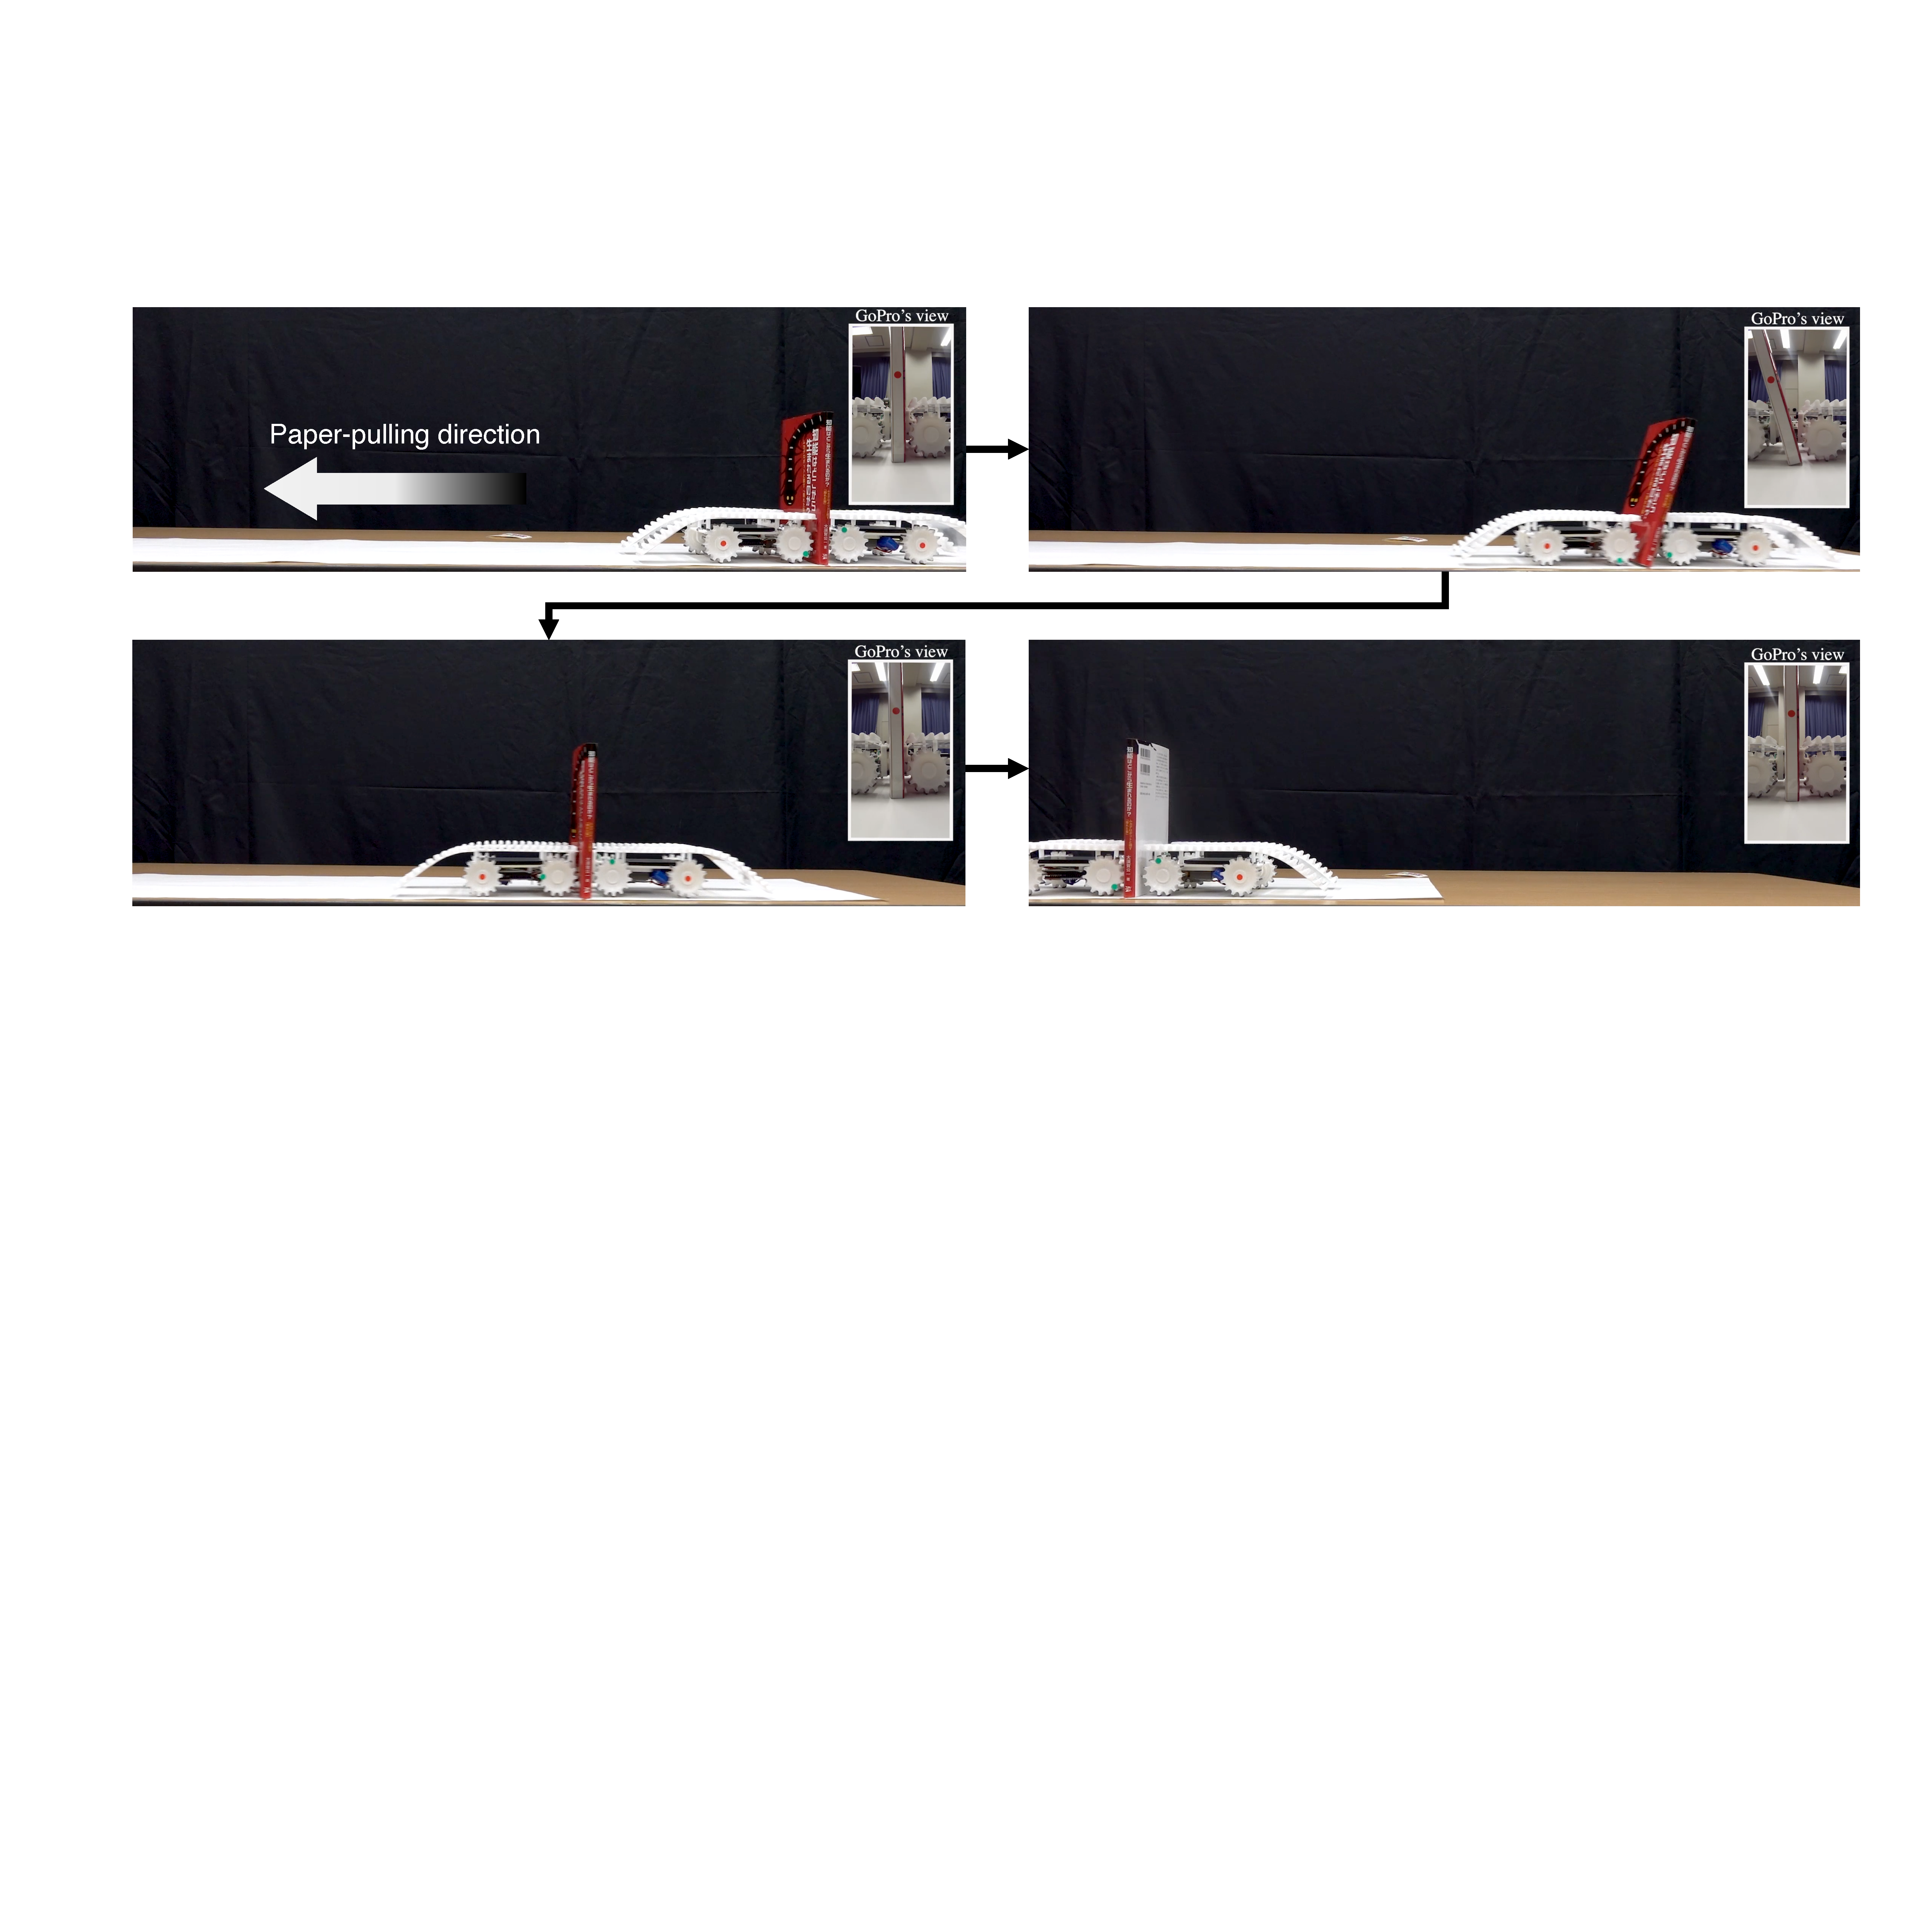
\includegraphics[width=\columnwidth]{figures/1layer-control.pdf}
  \caption{Experiment of applying control}
  \label{fig:control}
\end{figure}
\begin{figure}[tb]
  \centering
  \includegraphics[width=0.8\columnwidth]{figures/angle-control.eps}
  \caption{Angle of object}
  \label{fig:angle}
\end{figure}
\reffig{angle}には,制御ありとなしの比較したときの角度のグラフを示す.横軸は時間$t$,縦軸は物体の初期姿勢からの角度のずれ\si{\degree}である.ここで,物体の角度は進行方向の逆向きを正とする.制御なしの場合の角度は設定された$\pm3$\si{\degree}の範囲外にあることがわかった.一方,制御ありの場合は,$t=0$~sから$t=0.5$~sまでは,物体の初期姿勢から12\si{\degree}傾いたものの,$t=0.5$~s以降,物体の初期姿勢からの角度差は0に近づき,$\pm1.8$\si{\degree}範囲内に収めることがわかった.よって,制御をかけることで,ロボット1段でも支持することができると言える.その他,急に動き出すときの大きい角度差に対して,今後ロボットに搭載されている加速度センサを利用して,フィードフォワード制御をかけることで,より安定に運搬できると考えられる.